\documentclass{ieeeojies}
\usepackage{cite}
\usepackage{amsmath,amssymb,amsfonts}
\usepackage{algorithmic}
\usepackage{graphicx}
\usepackage{textcomp}
\usepackage{import}
%\graphicspath{{figures/}} %Setting the graphicspat%h
\graphicspath{{figures/}{figures/A/}{figures/B/}} %Setting the graphicspath
\makeatletter

%\providecommand*{\input@path}{}
%\edef\input@path{{figures/}{{figures/A/}{figures/B/}}\input@path}% prepend
\def\input@path{{figures/}{figures/A/}{figures/B/}}
\makeatother
\usepackage{subcaption}
\usepackage{multicol}

\usepackage{color}

\usepackage{listings}
\usepackage{amsthm}
\usepackage{stmaryrd}
\usepackage{amssymb}
\usepackage{wasysym}
\usepackage{array}
\usepackage{lipsum}  

\def\BibTeX{{\rm B\kern-.05em{\sc i\kern-.025em b}\kern-.08em
    T\kern-.1667em\lower.7ex\hbox{E}\kern-.125emX}}

\begin{document}
\title{Folded patch design}
\author{{Blasi Luca}\authorrefmark{1}, 
{Mastrofini Alessandro\authorrefmark{2}, and Mucenica Stefan}\authorrefmark{3},
}
\address[1]{National Institute of Standards and 
Technology, Boulder, CO 80305 USA (e-mail: author@boulder.nist.gov)}
\address[2]{Department of Physics, Colorado State University, Fort Collins, 
CO 80523 USA (e-mail: author@lamar.colostate.edu)}
\address[3]{Electrical Engineering Department, University of Colorado, Boulder, CO 
80309 USA}
\tfootnote{This work was developed for the Wireless Electromagnetic Technologies course held by Prof. G. Marrocco}





\begin{abstract}
These instructions give you guidelines for preparing papers for 
IEEE Open Journal of the Industrial Electronics Society. Use this document as a template if you are 
using \LaTeX. Otherwise, use this document as an 
instruction set. The electronic file of your paper will be formatted further 
at IEEE. Paper titles should be written in uppercase and lowercase letters, 
not all uppercase. Avoid writing long formulas with subscripts in the title; 
short formulas that identify the elements are fine (e.g., "Nd--Fe--B"). Do 
not write ``(Invited)'' in the title. Full names of authors are preferred in 
the author field, but are not required. Put a space between authors' 
initials. The abstract must be a concise yet comprehensive reflection of 
what is in your article. In particular, the abstract must be self-contained, 
without abbreviations, footnotes, or references. It should be a microcosm of 
the full article. The abstract must be between 150--250 words. Be sure that 
you adhere to these limits; otherwise, you will need to edit your abstract 
accordingly. The abstract must be written as one paragraph, and should not 
contain displayed mathematical equations or tabular material. The abstract 
should include three or four different keywords or phrases, as this will 
help readers to find it. It is important to avoid over-repetition of such 
phrases as this can result in a page being rejected by search engines. 
Ensure that your abstract reads well and is grammatically correct.
\end{abstract}

\begin{keywords}
antenna, antenna design, patch, folded patch, resonance, radiation, microwave
\end{keywords}

\titlepgskip=-15pt

\maketitle

\section{Introduction}
\label{sec:introduction}
WRITE INTRODUCTION 

\textcolor{blue}{\lipsum[1-4]}

\section{Tchebyshev array factor design}

The design of the Tchebyshev array factor will be made with five elements and a lobe/side lobe ratio of \textbf{R\,=\,41.58\,dB}. In order to minimize the beamwidth, let's look for the optimal inter-spacing:

\begin{equation}
	\begin{split}
	d_{\max}\,=\,\lambda\,\left[1-\frac{1}{2\pi}\,\arccos\left(\frac{3\,-\,x_1}{1\,+\,x_1}\right)\right]
	\\ \text{with}\quad d_{\max}\,\in\,\left[\frac{\lambda}{2}\,,\,\lambda\right]
	\end{split}
\end{equation}

\begin{table}[bt!]
	\centering
	\begin{tabular}{|c|c|}
		\hline
		{Parameter}& {Value} \\
		\hline
		{Feed coefficients} $[A]$ &  \footnotesize{$\begin{bmatrix}
				C_{-2}\\
				C_{-1}\\
				C_0\\
				C_1\\
				C_2\\
			\end{bmatrix}\,=\,\begin{bmatrix}
				9.6\\
				29.8\\
				41.2\\
				29.8\\
				9.6\\
			\end{bmatrix}$}\\
		\hline 	\\[-1em]
		{Tapering efficiency} & \footnotesize{$\eta_T\,=\,79\,\%$}\\ 
		\hline 
		{Beamwidth} & 
		 \begin{tabular}{c| c}
			{Tchebyshev} & {Uniform} \\
				$50.6^\circ$ &$ 34.8^\circ $ \\
		\end{tabular}  \\
		\hline 
	\end{tabular}

\caption{Parametri materiali}\label{tab:example}
\end{table}




\begin{center}
	\begin{figure*}[t]
			\begin{subfigure}[t]{0.38\textwidth}
  	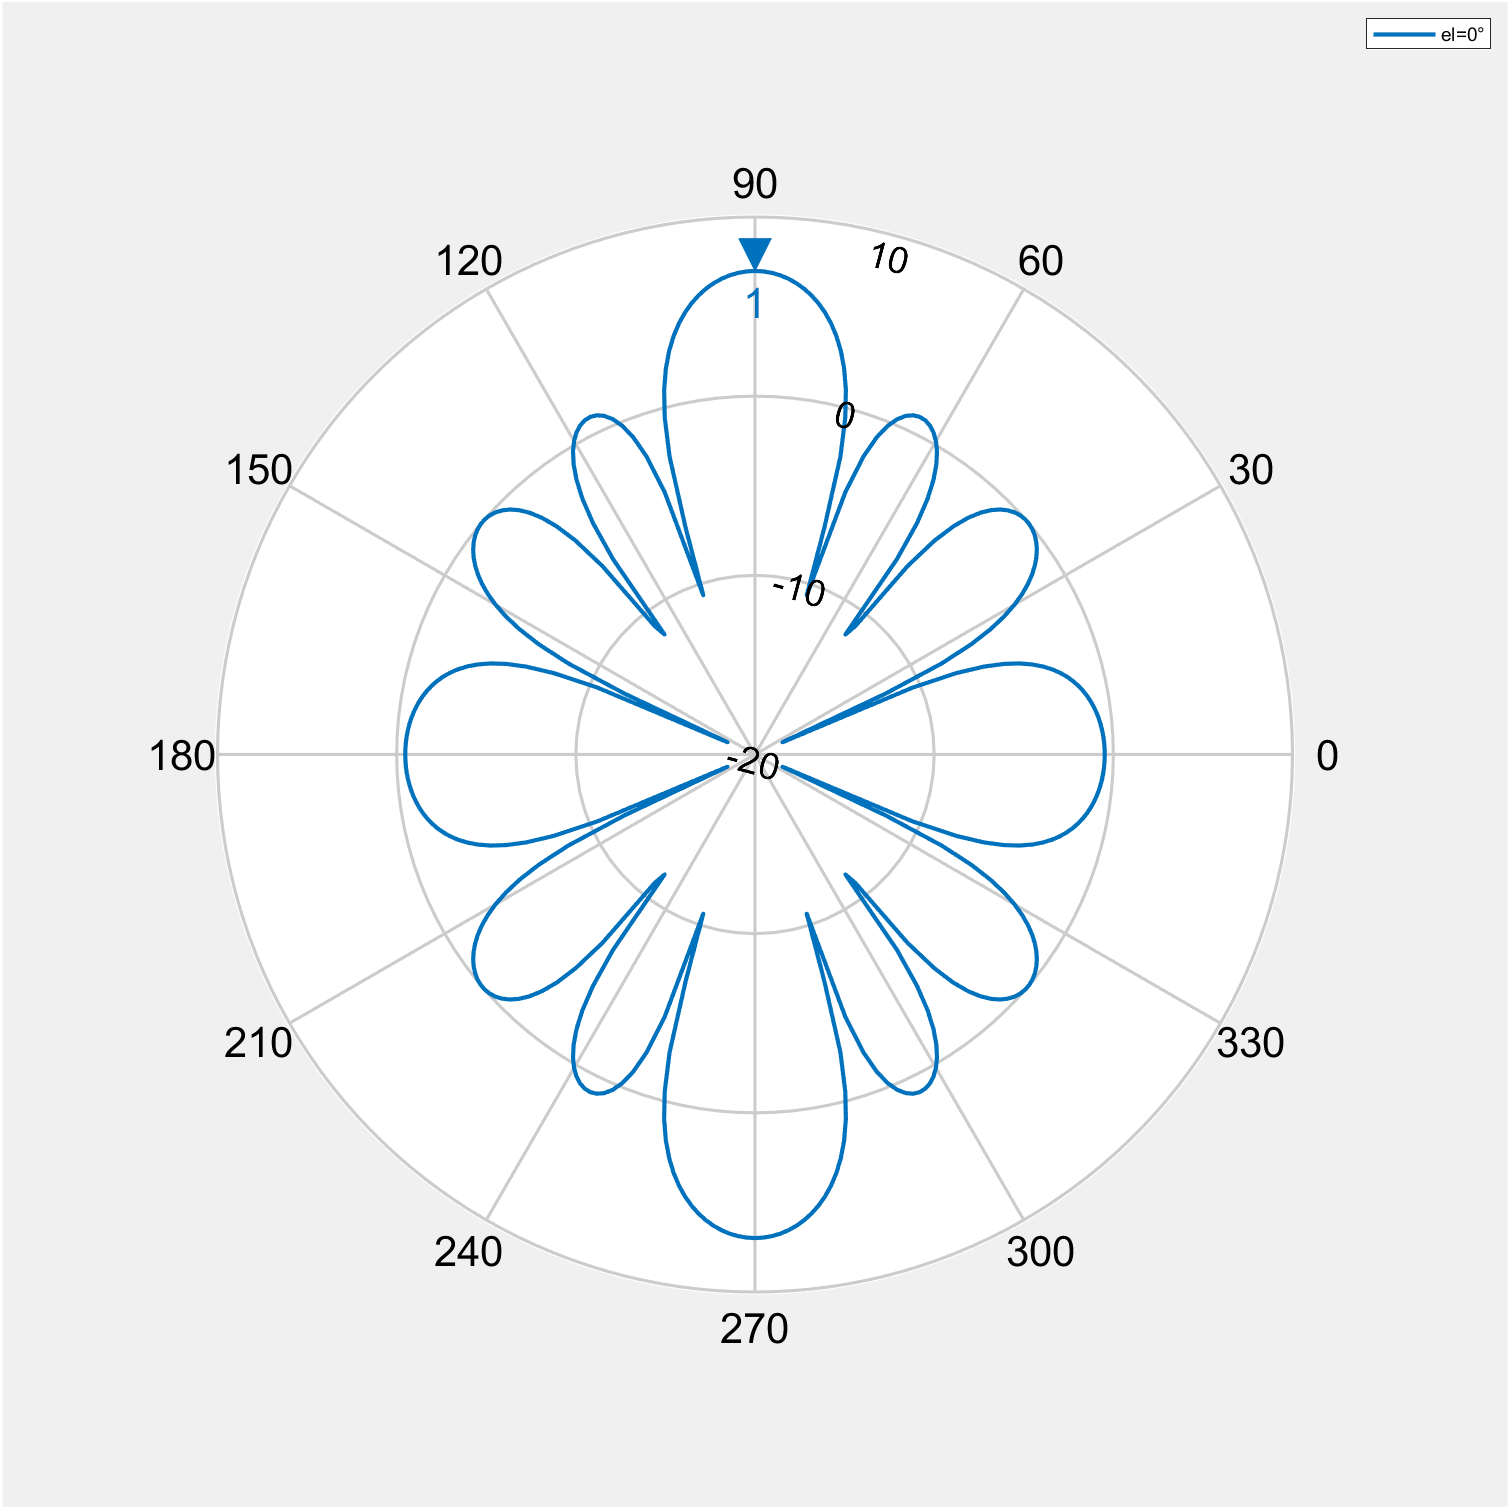
\includegraphics[width=\textwidth]{array_factor_polar.png}
  	  \subcaption{ }
	\end{subfigure}
	\begin{subfigure}[t]{0.62\textwidth}
		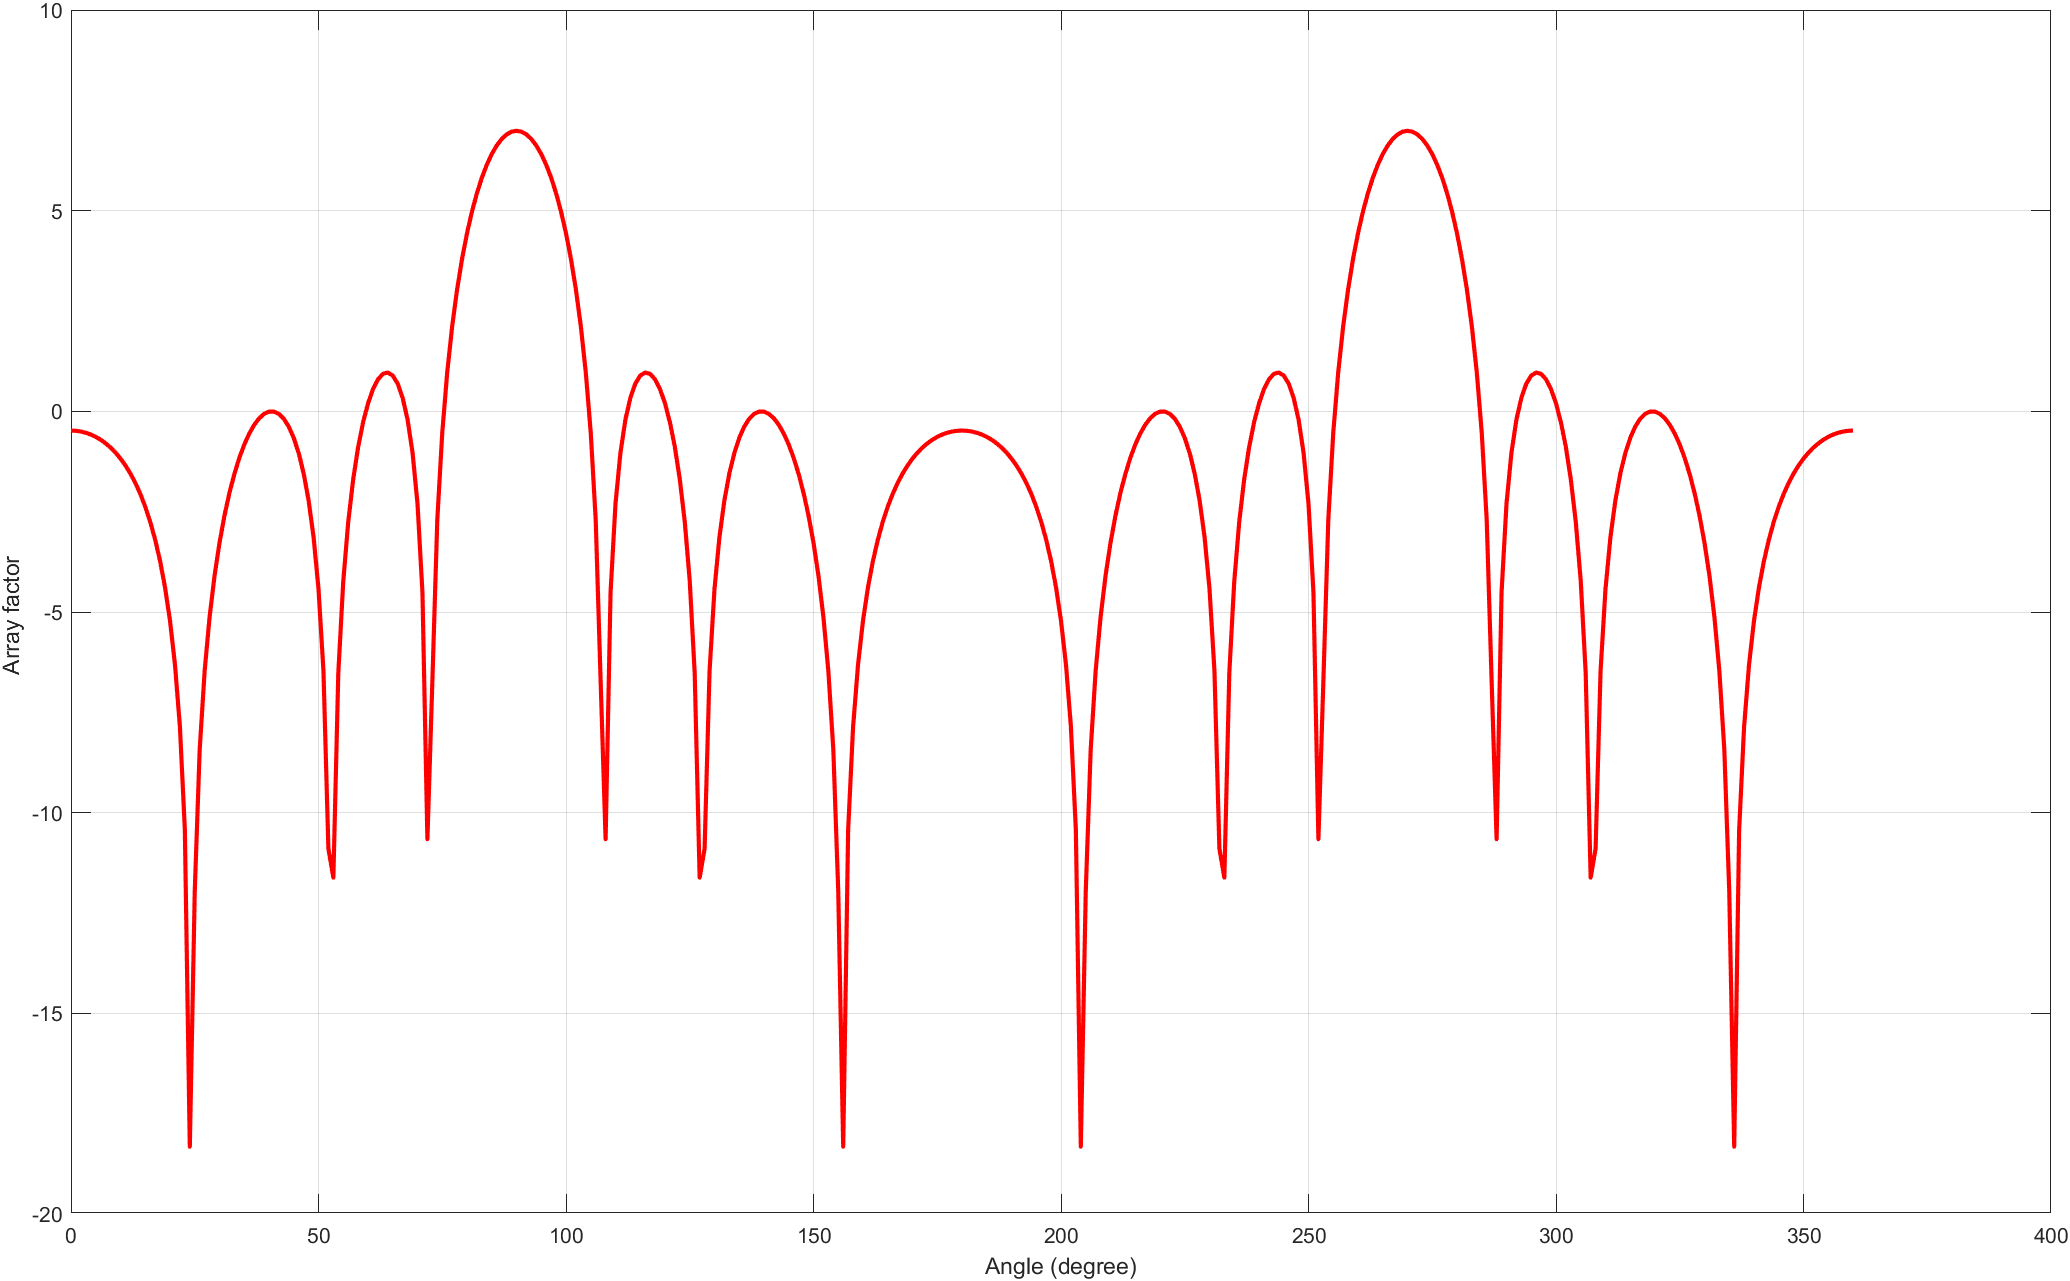
\includegraphics[width=\textwidth]{array_factor_rectangular.png}
  	  \subcaption{ }
	\end{subfigure}
		\caption{ Array factor polar (a) and rectangular (b) diagrams}
	\end{figure*}
\end{center}



\section{Rectangular folded patch design}
\subsection{Mesh density refinement}

A FR4 substrate thickness of $h_{sub}\,=\,0.8\,mm$  has been selected so it could be considered as a thin one:
\[\lambda_{sub}\,=\,0.0652\,m\quad \leadsto\quad \frac{h_{sub}}{\lambda_{sub}}\,\cong\,\frac{1}{81}\]
In case of thin substrates ($h/\lambda\,\leq\,1/50$),  the \texttt{Antenna Toolbox} suggests to mesh the antenna using dielectric in auto mode. The other two available substrate thicknesses ($1.0\,mm$ and $1.6\,mm$) have not been adopted because the \texttt{Antenna Toolbox} reference doesn't give any information about accuracy of the results in case of $h_{sub}\,\in\,\left(\frac{\lambda}{50}\,,\,\frac{\lambda}{10}\right)$. 
\begin{center}
	\begin{figure}[h]
		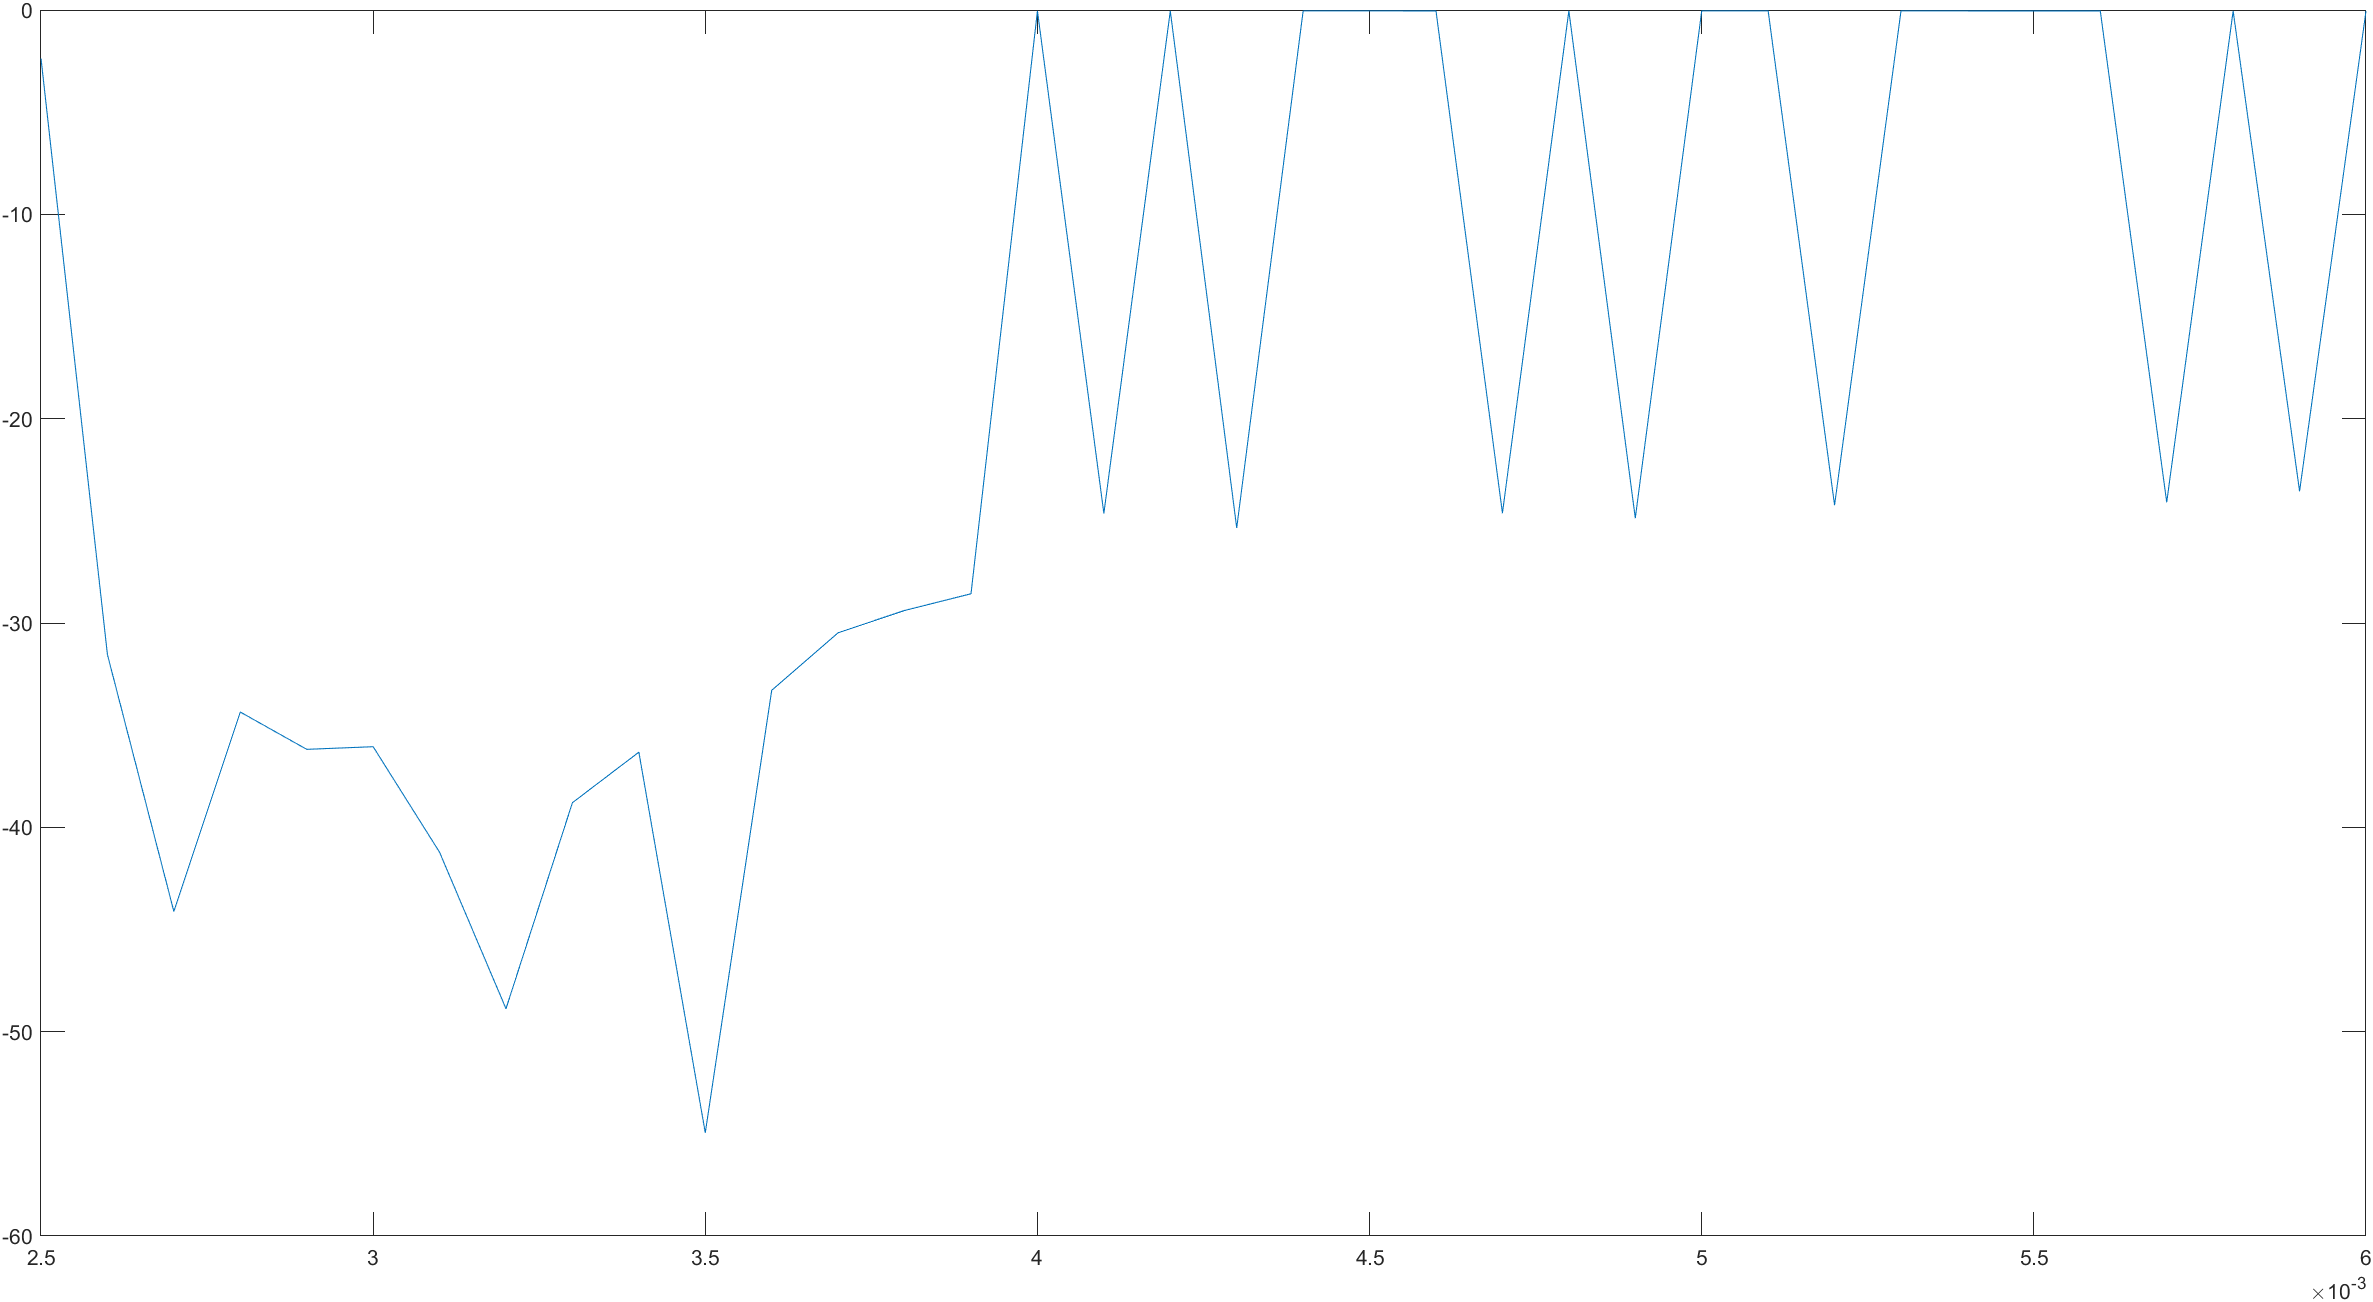
\includegraphics[width=0.48\textwidth]{mesh_levels.png}
		\caption{{ Minimum of the reflection coefficient $\Gamma\, \text{[dB]}$ in the frequency range $2.0\div 2.2\,\text{GHz}$ depending on the varying mesh density level}}
	\end{figure}
\end{center}
\subsection{Patch parameters}
\begin{subequations}
	\begin{align}L\,+\,W\,-\,w_{SC}\,&{=}\,\frac{\lambda}{4}\,+\,h_{sub}\\
		W\,&{=}\,\frac{\lambda_0}{2}\,\sqrt{\frac{2}{\varepsilon_r\,+\,1}}
	\end{align}
\end{subequations}
\begin{subequations}
	\begin{align}
		BW_E\,&{=}\,2\,\arccos\,\sqrt{\frac{7.03\,\lambda_0^2}{4\,(3\,L_e^2+h^2)\,\pi^2}}\\
		BW_H\,&{=}\,2\,\arccos\sqrt{\frac{1}{2\,+\,k_0\,W}}
	\end{align}
\end{subequations}
\begin{equation}
	\ell_{\operatorname{feed}}\,{=}\,\frac{L}{\pi}\,\arccos\,\sqrt{\frac{R_{in}}{R_r}}
\end{equation}
%% w_{feed} = 0.001 

\begin{center}
	\begin{figure*}[t]
			\begin{subfigure}[t]{0.32\textwidth}
		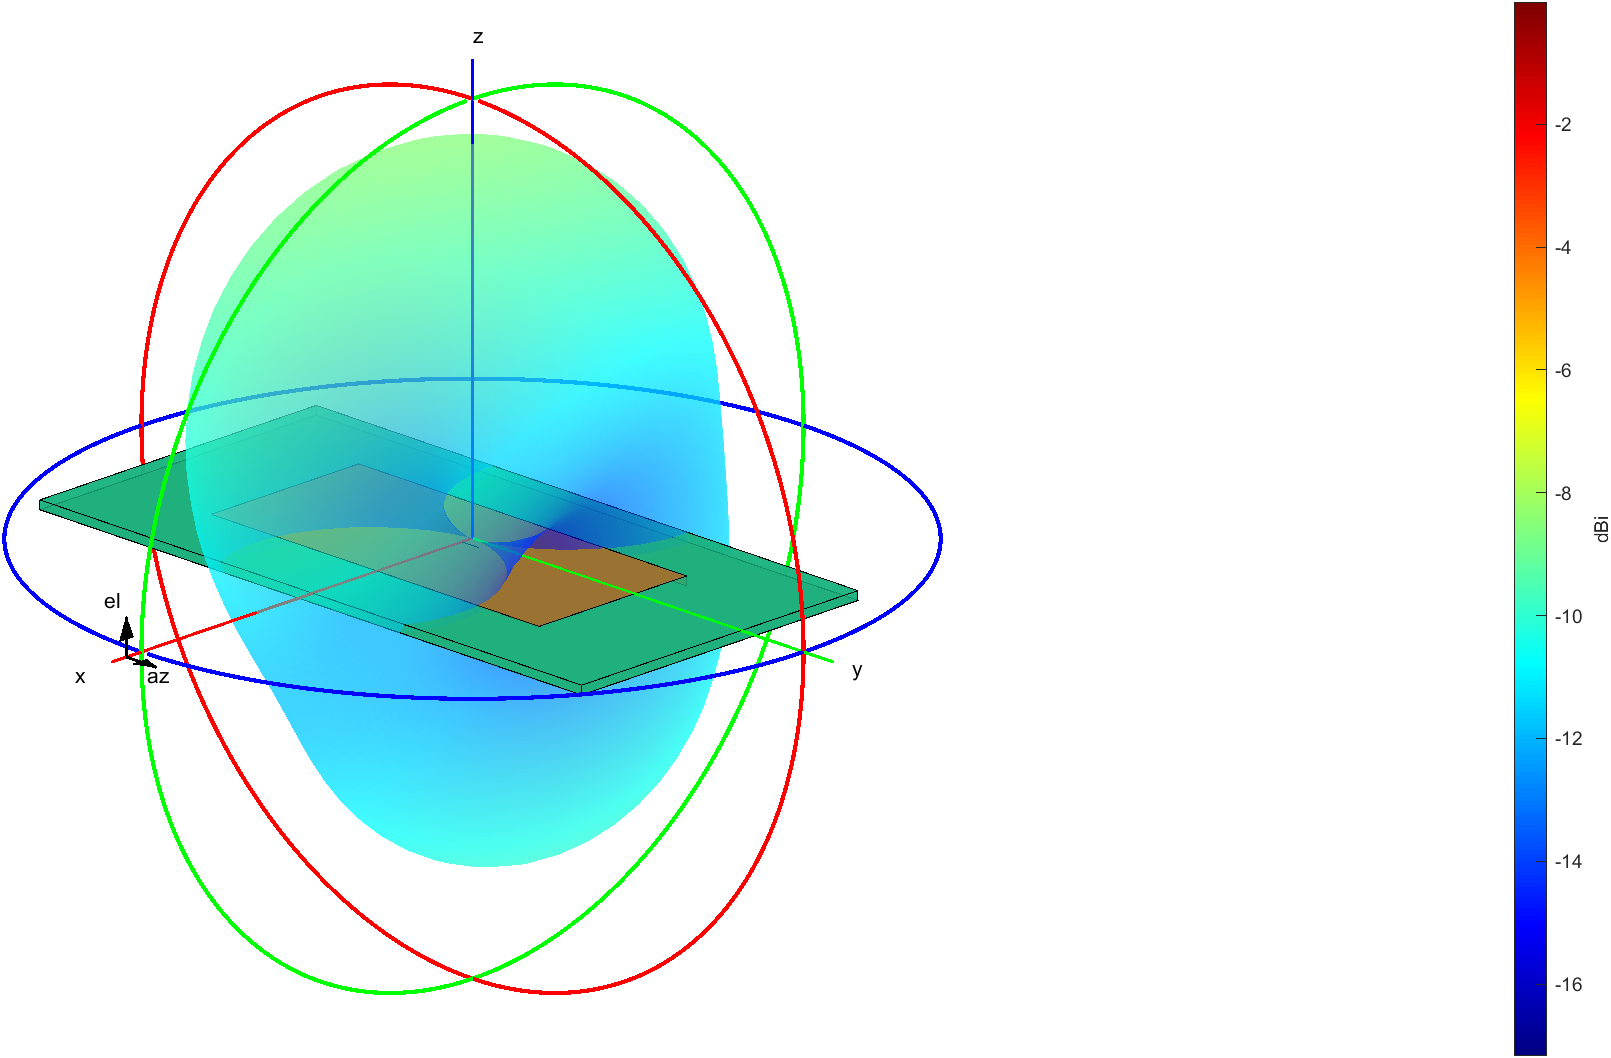
\includegraphics[width = \linewidth]{gain_patch.png}
				\subcaption{}
	\end{subfigure}
	\begin{subfigure}[t]{0.32\textwidth}
		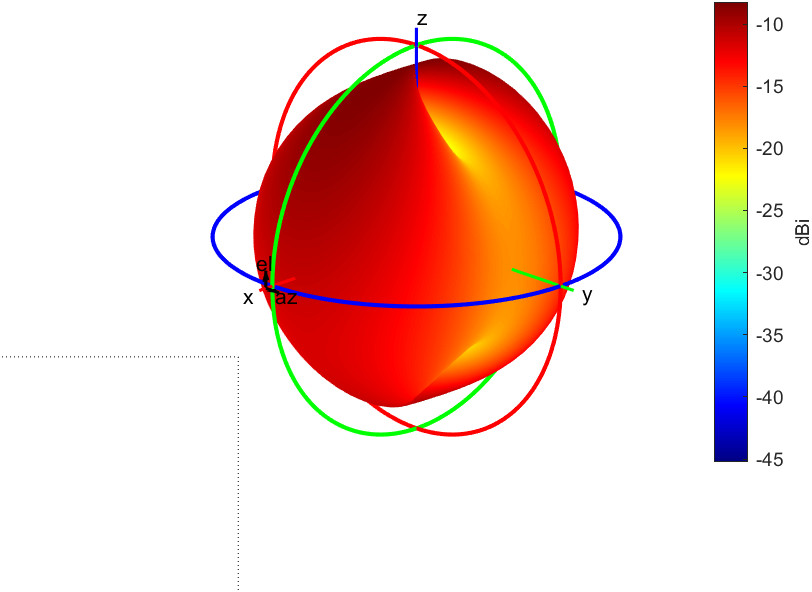
\includegraphics[width = \linewidth]{gain_patch_v.png}
						\subcaption{}
	\end{subfigure}
	\begin{subfigure}[t]{0.32\textwidth}
		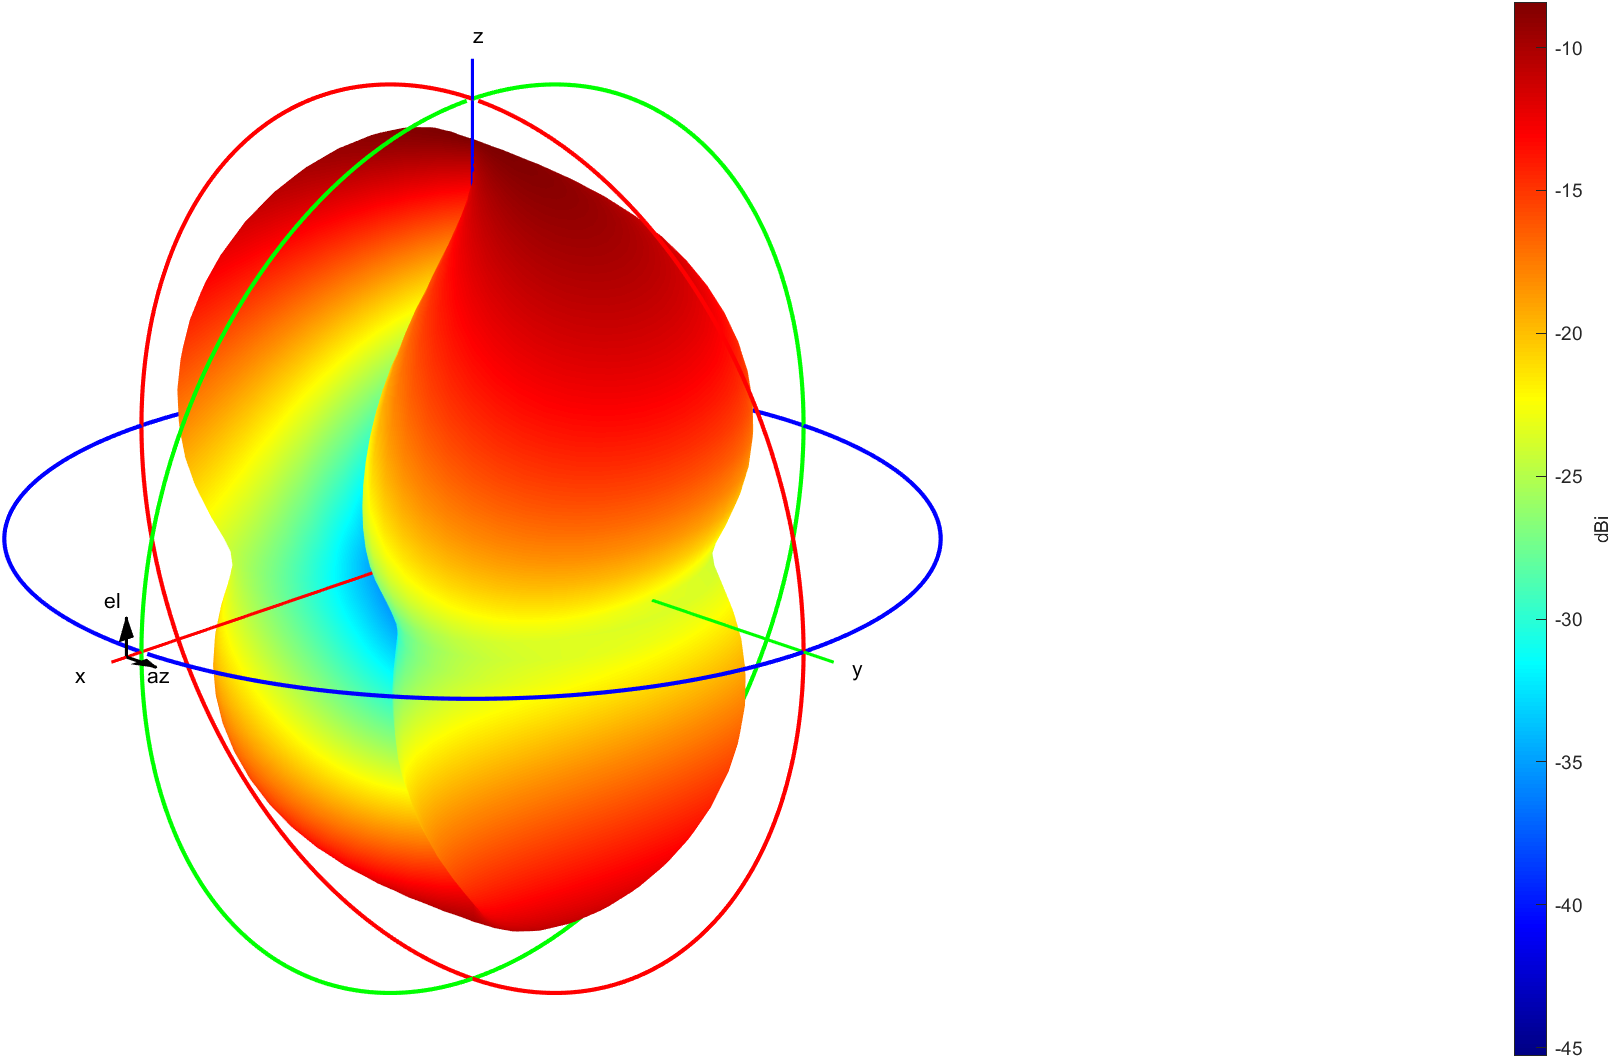
\includegraphics[width = \linewidth]{gain_patch_h.png}
						\subcaption{}
	\end{subfigure}
		\caption{ Gain pattern (a), gain pattern with vertical polarization (b) and with the horizontal one (c)}
	\end{figure*}
\end{center}


\begin{center}
	\begin{figure*}[t]
			\begin{subfigure}[t]{0.5\textwidth}
		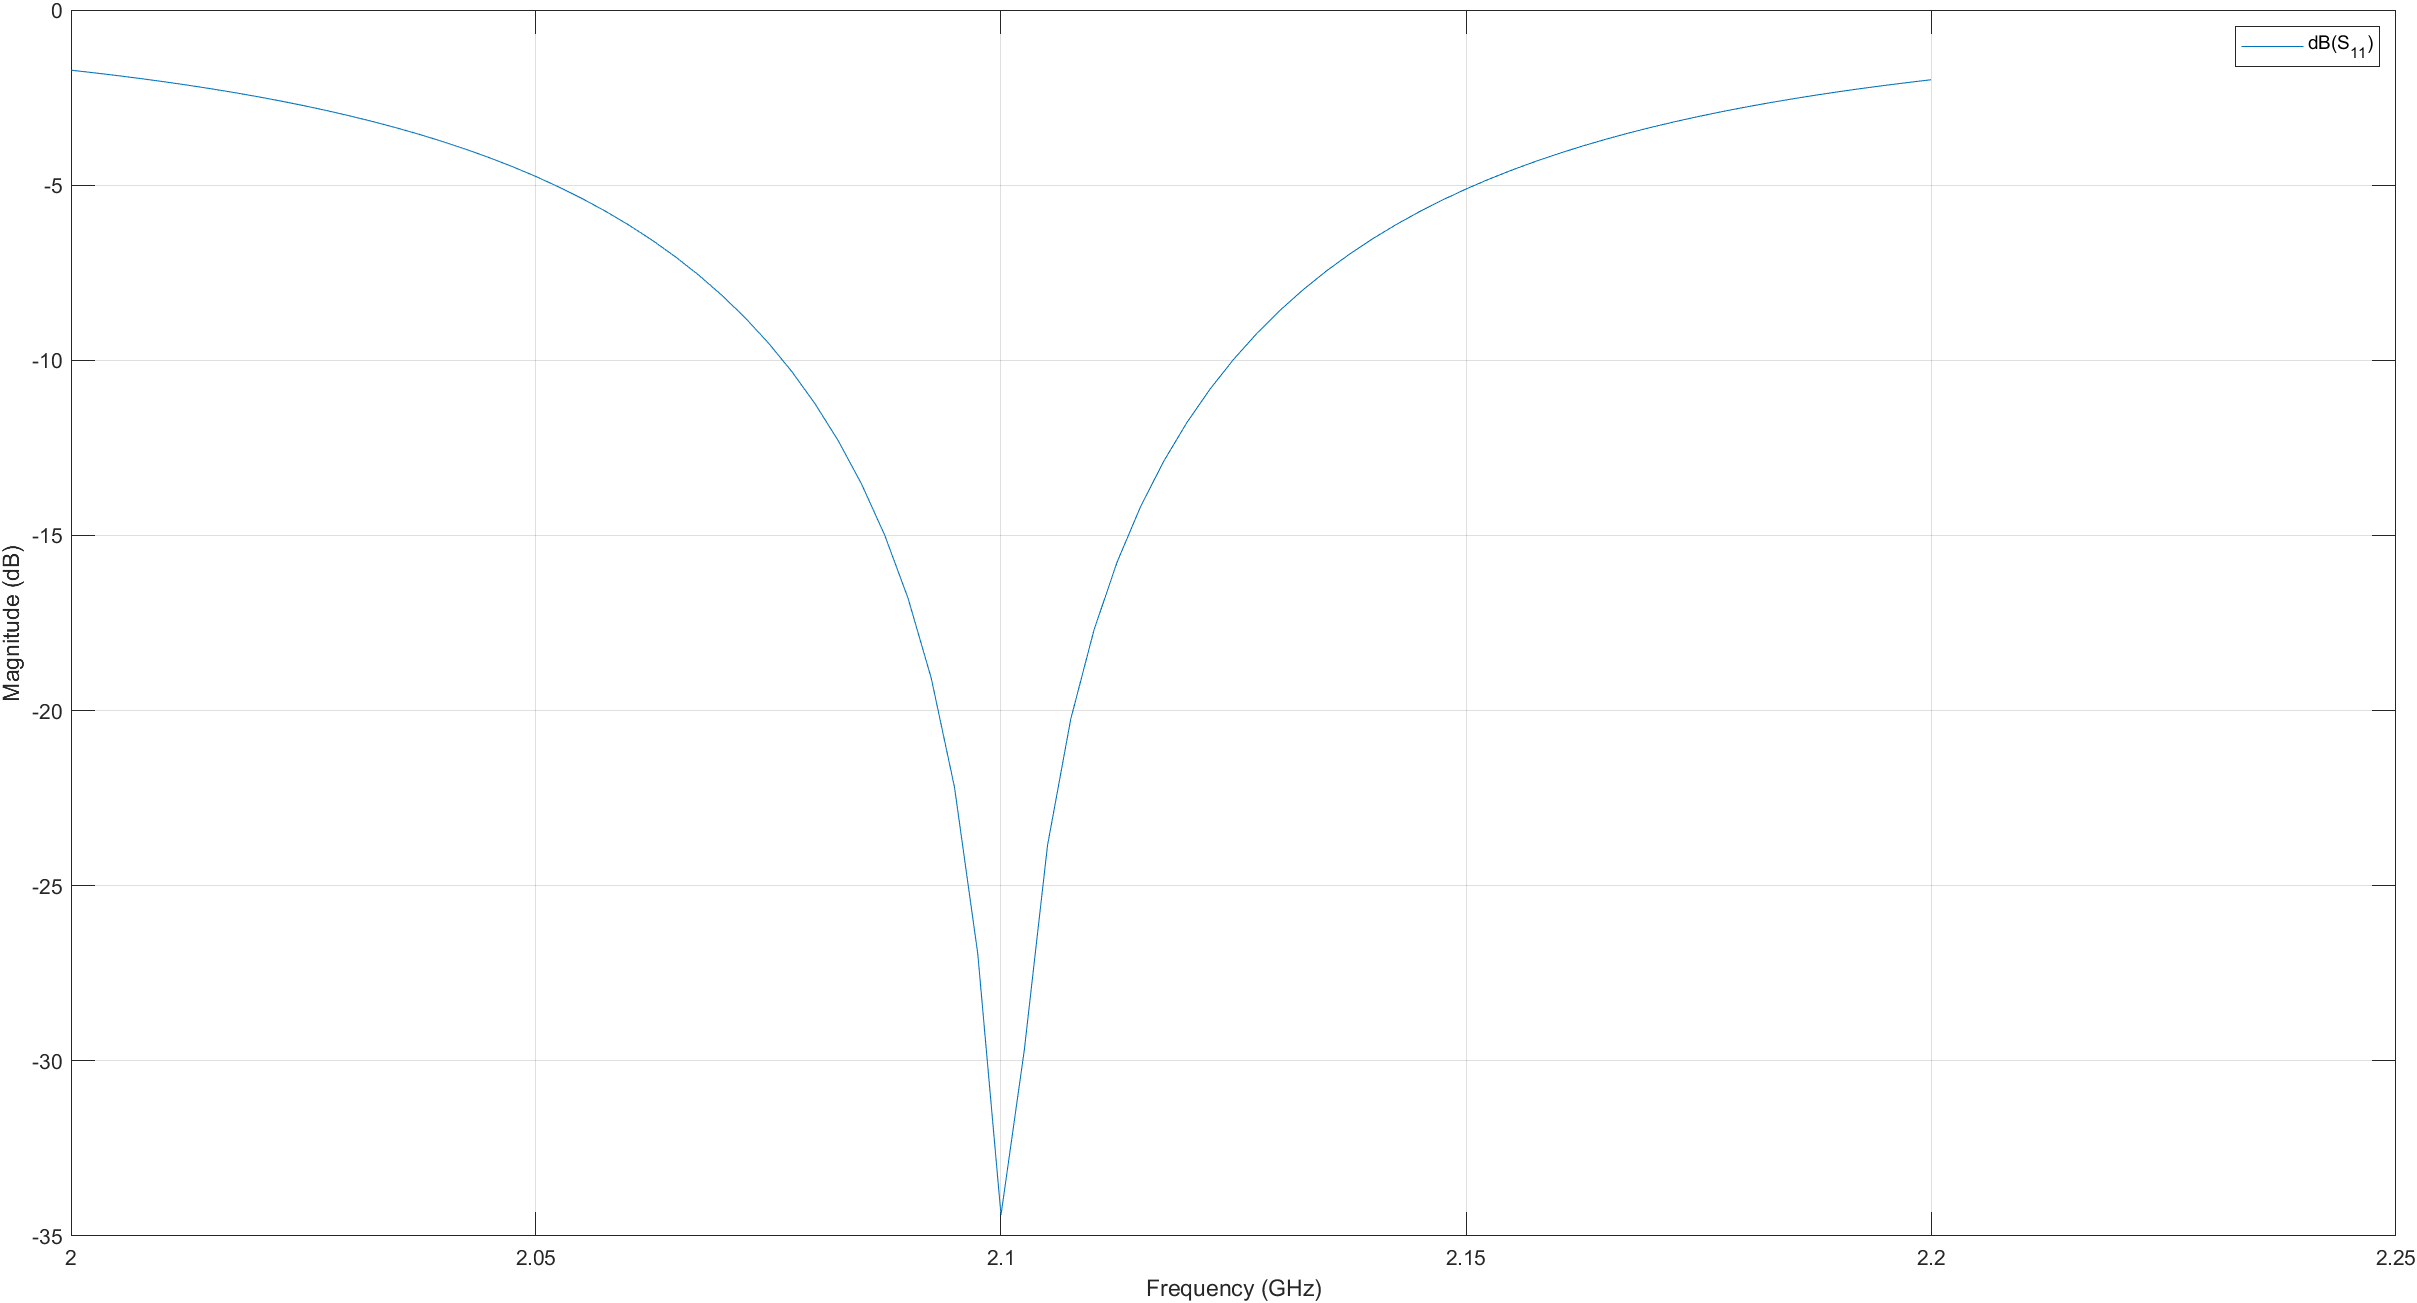
\includegraphics[width = \linewidth]{gamma.png}
								\subcaption{}
	\end{subfigure}
	\begin{subfigure}[t]{0.5\textwidth}
		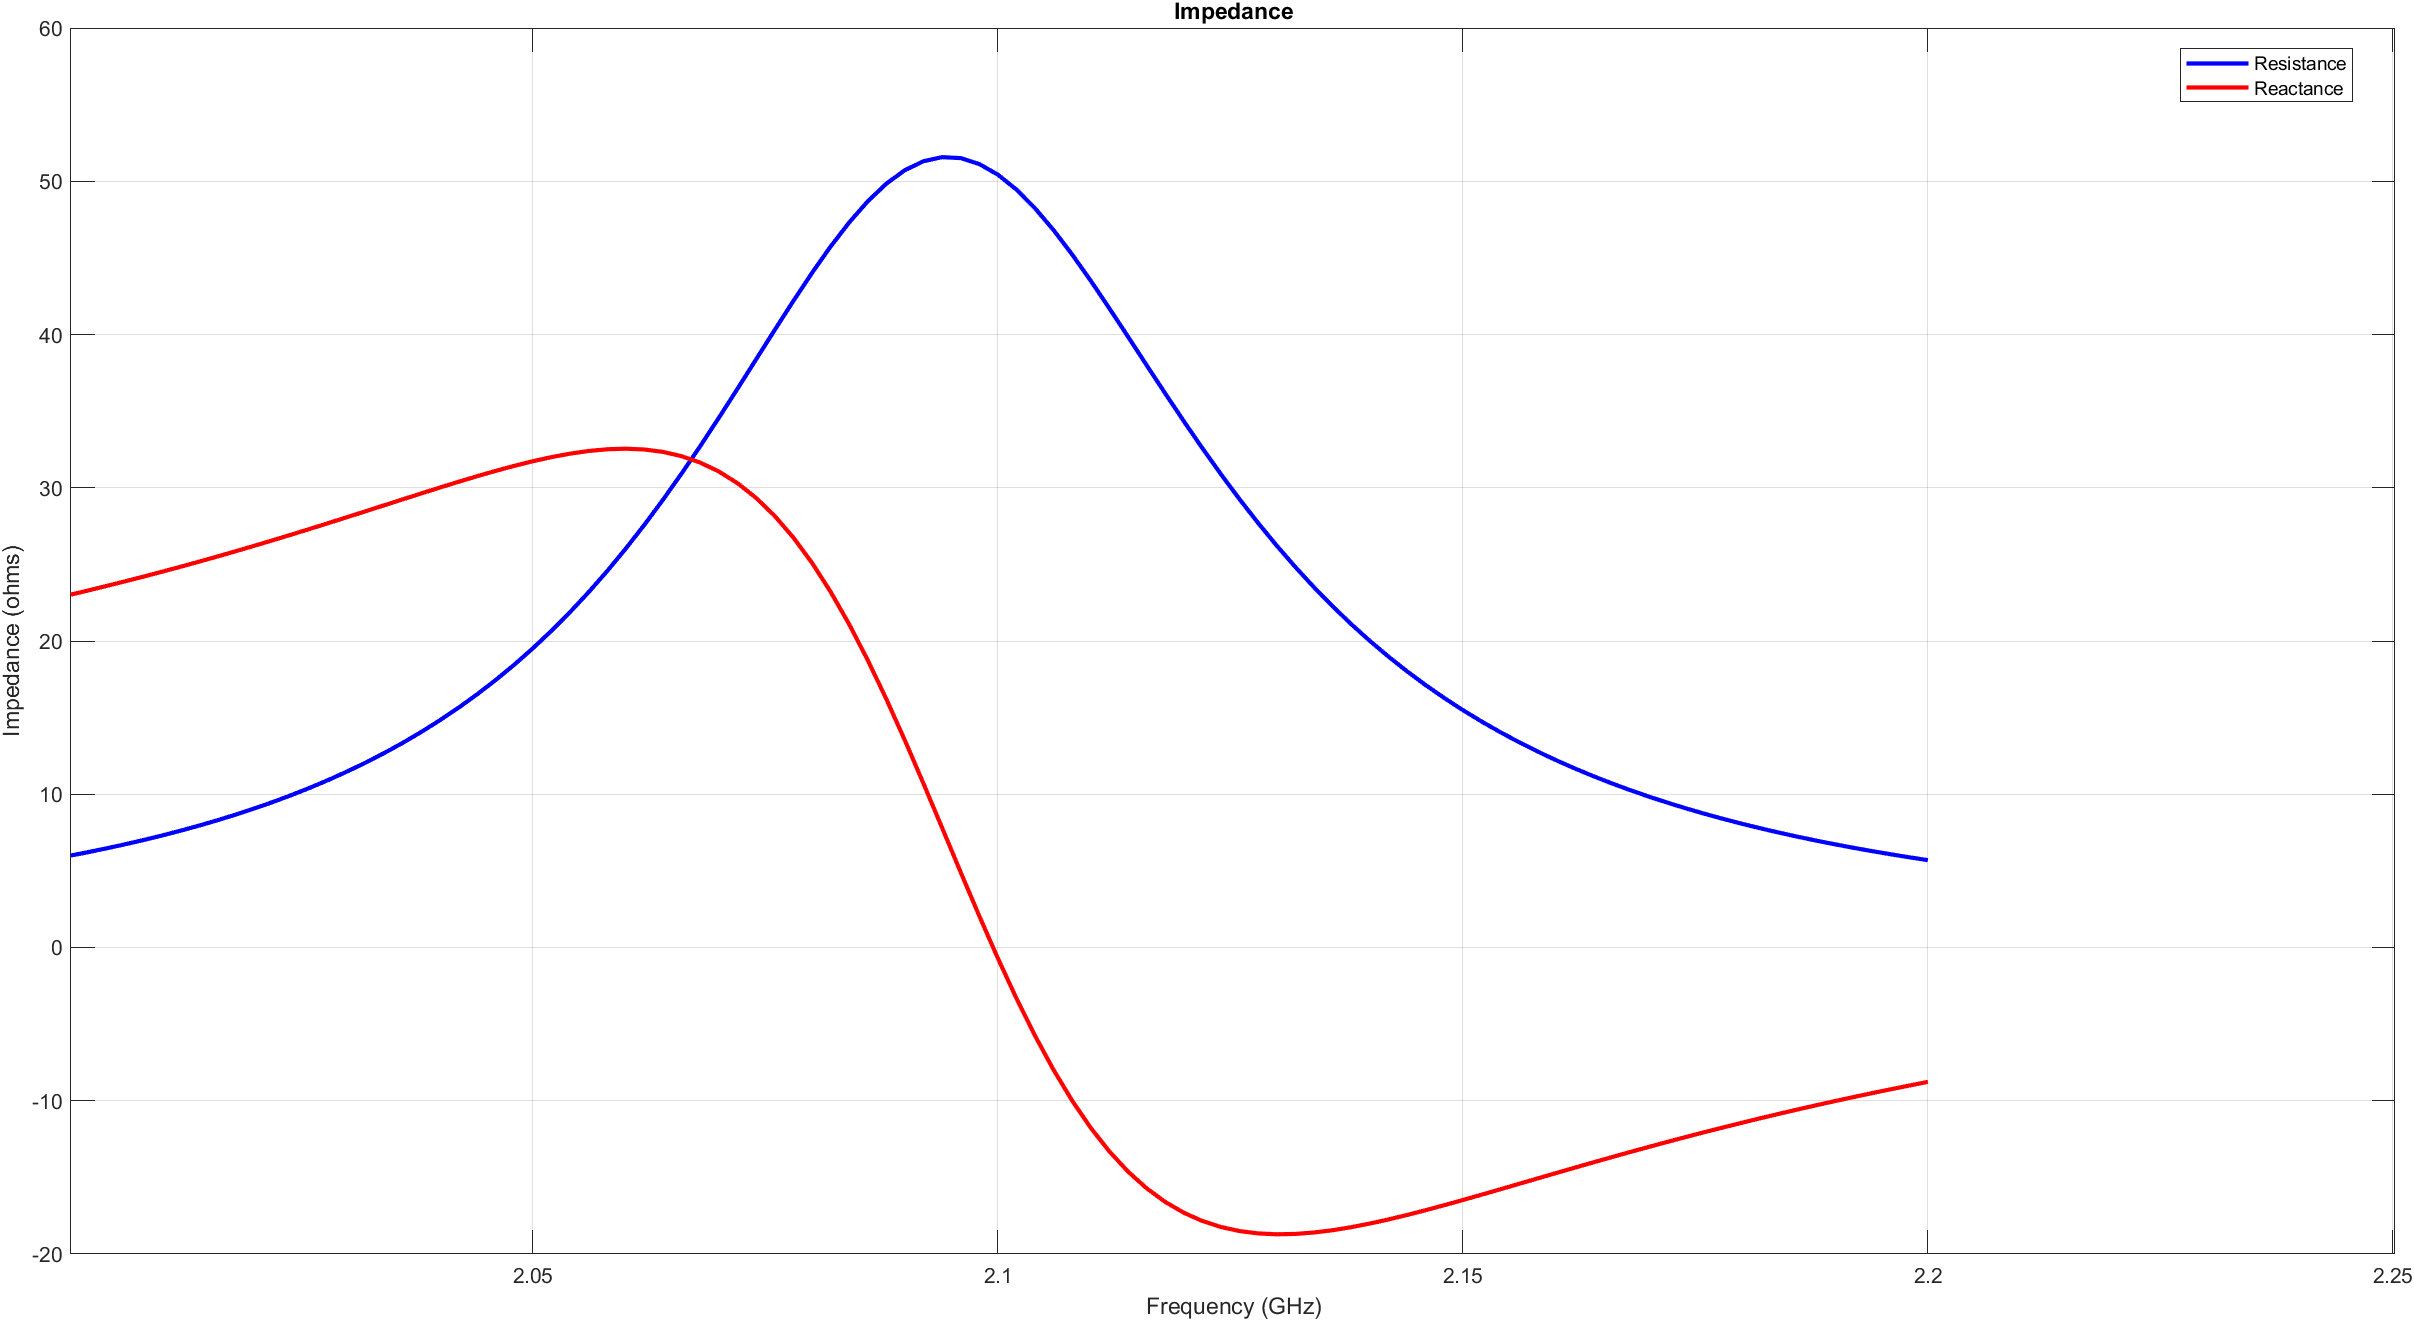
\includegraphics[width = \linewidth]{impedances.png}
						\subcaption{}		
	\end{subfigure}
		\caption{ Reflection coefficient (left) and impedances (right) plots depending on $f\,\in\,2.0\div 2.1\,\text{GHz}$}
	\end{figure*}
\end{center}
\begin{center}
	\begin{figure*}[t]
		\begin{subfigure}[t]{0.5\textwidth}
			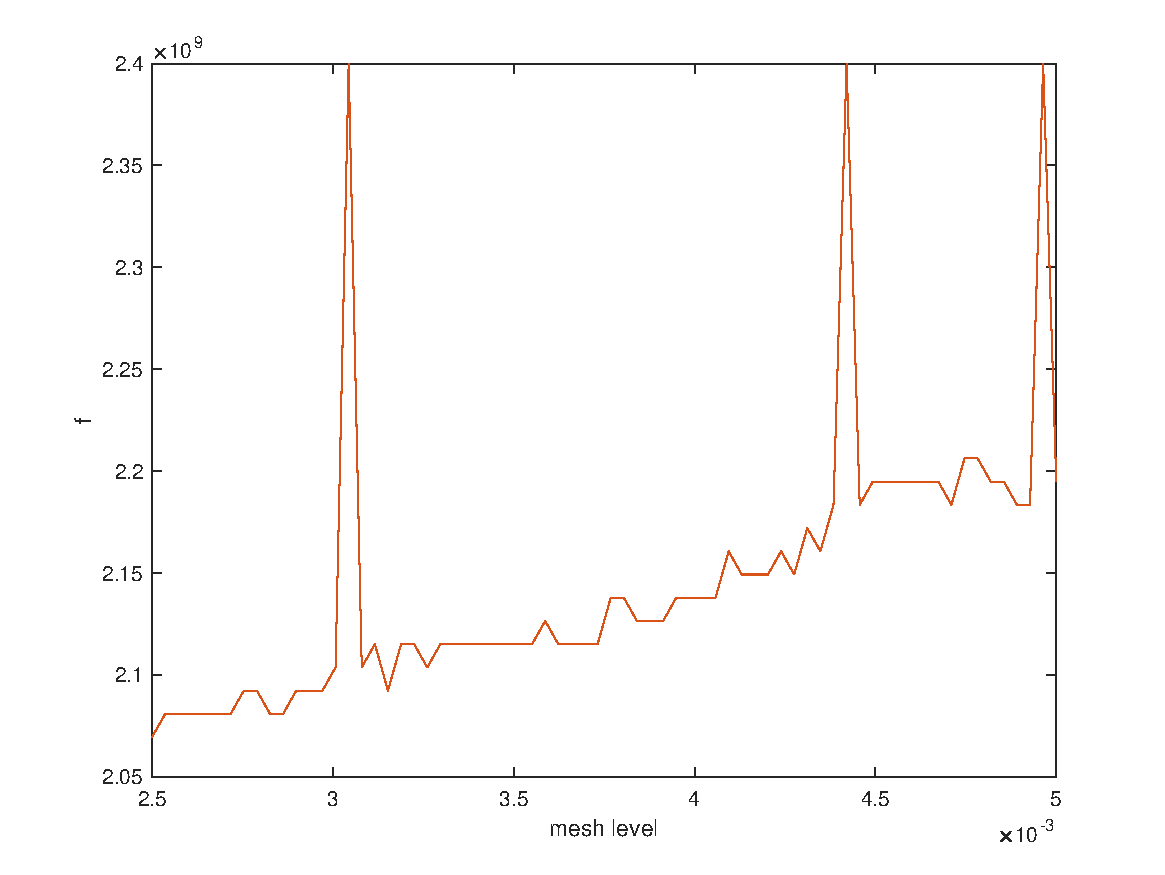
\includegraphics[width = \linewidth]{/B/F_vs_mesh_level.pdf}
			\subcaption{}
		\end{subfigure}
		\begin{subfigure}[t]{0.5\textwidth}
			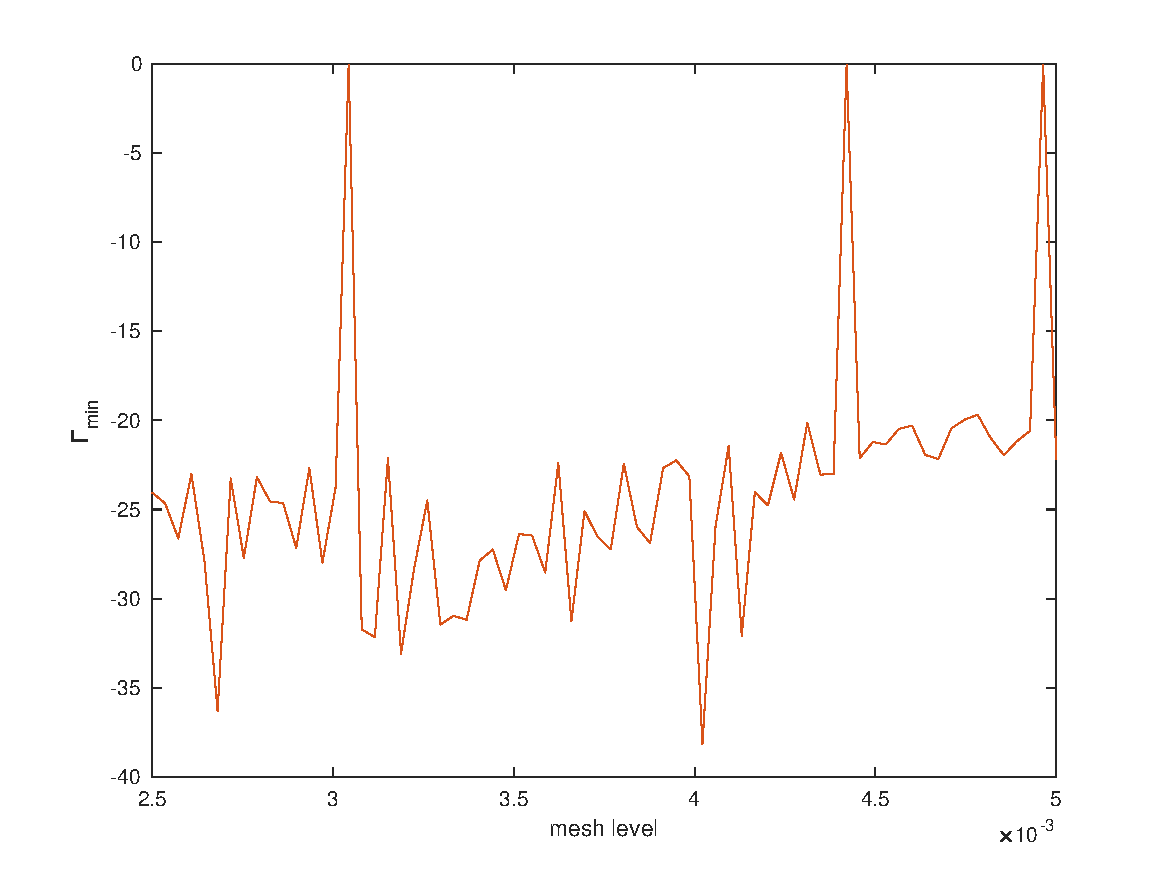
\includegraphics[width = \linewidth]{minGamma_vs_mesh_level.pdf}
			\subcaption{}		
		\end{subfigure}
	
	\end{figure*}
\end{center}
\subsection{Overall array performance evaluation}

\begin{center}
	\begin{figure}[t]
	\def\svgwidth{\linewidth}
	\small{\input{Array_Factor_Azimuth_Pattern_Polar_Coordinates_tex.pdf_tex}}
\caption{Polar pattern in azimuth cut for the array factor of the Tchebyshef array (CITA SEZIONE). The maximus is identified by the (*) peak of 4.639 dB.}	
\end{figure}
\end{center}

\begin{center}
	\begin{figure}[t]
		\def\svgwidth{\linewidth}
		\small{\input{Array_Factor_Azimuth_Pattern_Rectangular_Coordinates_tex.pdf_tex}}
		\caption{Rectangular pattern of the array factor of the Tchebyshef array (CITA SEZIONE).}	
	\end{figure}
\end{center}

\begin{center}
	\begin{figure*}[t]
		\def\svgwidth{\linewidth}
		\small{\input{Second_Contour_LOG_tex.pdf_tex}}
		\caption{Rectangular pattern of the array factor of the Tchebyshef array (CITA SEZIONE).}	
	\end{figure*}
\end{center}

\section{Reference Examples}

\begin{itemize}

\item \emph{Basic format for books:}\\
J. K. Author, ``Title of chapter in the book,'' in \emph{Title of His Published Book, x}th ed. City of Publisher, (only U.S. State), Country: Abbrev. of Publisher, year, ch. $x$, sec. $x$, pp. \emph{xxx--xxx.}\\
See \cite{b1,b2}.

\item \emph{Basic format for periodicals:}\\
J. K. Author, ``Name of paper,'' \emph{Abbrev. Title of Periodical}, vol. \emph{x, no}. $x, $pp\emph{. xxx--xxx, }Abbrev. Month, year, DOI. 10.1109.\emph{XXX}.123456.\\
See \cite{b3}--\cite{b5}.

\item \emph{Basic format for reports:}\\
J. K. Author, ``Title of report,'' Abbrev. Name of Co., City of Co., Abbrev. State, Country, Rep. \emph{xxx}, year.\\
See \cite{b6,b7}.

\item \emph{Basic format for handbooks:}\\
\emph{Name of Manual/Handbook, x} ed., Abbrev. Name of Co., City of Co., Abbrev. State, Country, year, pp. \emph{xxx--xxx.}\\
See \cite{b8,b9}.

\item \emph{Basic format for books (when available online):}\\
J. K. Author, ``Title of chapter in the book,'' in \emph{Title of
Published Book}, $x$th ed. City of Publisher, State, Country: Abbrev.
of Publisher, year, ch. $x$, sec. $x$, pp. \emph{xxx--xxx}. [Online].
Available: \underline{http://www.web.com}\\
See \cite{b10}--\cite{b13}.

\item \emph{Basic format for journals (when available online):}\\
J. K. Author, ``Name of paper,'' \emph{Abbrev. Title of Periodical}, vol. $x$, no. $x$, pp. \emph{xxx--xxx}, Abbrev. Month, year. Accessed on: Month, Day, year, DOI: 10.1109.\emph{XXX}.123456, [Online].\\
See \cite{b14}--\cite{b16}.

\item \emph{Basic format for papers presented at conferences (when available online): }\\
J.K. Author. (year, month). Title. presented at abbrev. conference title. [Type of Medium]. Available: site/path/file\\
See \cite{b17}.

\item \emph{Basic format for reports and handbooks (when available online):}\\
J. K. Author. ``Title of report,'' Company. City, State, Country. Rep. no., (optional: vol./issue), Date. [Online] Available: site/path/file\\
See \cite{b18,b19}.

\item \emph{Basic format for computer programs and electronic documents (when available online): }\\
Legislative body. Number of Congress, Session. (year, month day). \emph{Number of bill or resolution}, \emph{Title}. [Type of medium]. Available: site/path/file\\
\textbf{\emph{NOTE: }ISO recommends that capitalization follow the accepted practice for the language or script in which the information is given.}\\
See \cite{b20}.

\item \emph{Basic format for patents (when available online):}\\
Name of the invention, by inventor's name. (year, month day). Patent Number [Type of medium]. Available: site/path/file\\
See \cite{b21}.

\item \emph{Basic format}\emph{for conference proceedings (published):}\\
J. K. Author, ``Title of paper,'' in \emph{Abbreviated Name of Conf.}, City of Conf., Abbrev. State (if given), Country, year, pp. \emph{xxxxxx.}\\
See \cite{b22}.

\item \emph{Example for papers presented at conferences (unpublished):}\\
See \cite{b23}.

\item \emph{Basic format for patents}$:$\\
J. K. Author, ``Title of patent,'' U.S. Patent \emph{x xxx xxx}, Abbrev. Month, day, year.\\
See \cite{b24}.

\item \emph{Basic format for theses (M.S.) and dissertations (Ph.D.):}
\begin{enumerate}
\item J. K. Author, ``Title of thesis,'' M.S. thesis, Abbrev. Dept., Abbrev. Univ., City of Univ., Abbrev. State, year.
\item J. K. Author, ``Title of dissertation,'' Ph.D. dissertation, Abbrev. Dept., Abbrev. Univ., City of Univ., Abbrev. State, year.
\end{enumerate}
See \cite{b25,b26}.

\item \emph{Basic format for the most common types of unpublished references:}
\begin{enumerate}
\item J. K. Author, private communication, Abbrev. Month, year.
\item J. K. Author, ``Title of paper,'' unpublished.
\item J. K. Author, ``Title of paper,'' to be published.
\end{enumerate}
See \cite{b27}--\cite{b29}.

\item \emph{Basic formats for standards:}
\begin{enumerate}
\item \emph{Title of Standard}, Standard number, date.
\item \emph{Title of Standard}, Standard number, Corporate author, location, date.
\end{enumerate}
See \cite{b30,b31}.

\item \emph{Article number in~reference examples:}\\
See \cite{b32,b33}.

\item \emph{Example when using et al.:}\\
See \cite{b34}.

\end{itemize}


%% these lines used to import a separate ".bib" for the bibliografy.
\bibliographystyle{bibliography/IEEEtranIES}
\bibliography{bibliography/IEEEabrv,bibliography/mybibfile}

%% UNCOMMENT these lines below (and remove the 2 commands above) if you want to embed the bibliografy.
%\begin{thebibliography}{00}
%\bibitem{b1} G. O. Young, ``Synthetic structure of industrial plastics,'' in \emph{Plastics,} 2\textsuperscript{nd} ed., vol. 3, J. Peters, Ed. New York, NY, USA: McGraw-Hill, 1964, pp. 15--64. 
%\bibitem{b2} W.-K. Chen, \emph{Linear Networks and Systems.} Belmont, CA, USA: Wadsworth, 1993, pp. 123--135. 
%\bibitem{b3} J. U. Duncombe, ``Infrared navigation---Part I: An assessment of feasibility,'' \emph{IEEE Trans. Electron Devices}, vol. ED-11, no. 1, pp. 34--39, Jan. 1959, 10.1109/TED.2016.2628402. 
%\bibitem{b4} E. P. Wigner, ``Theory of traveling-wave optical laser,'' \emph{Phys. Rev}., vol. 134, pp. A635--A646, Dec. 1965. 
%\bibitem{b5} E. H. Miller, ``A note on reflector arrays,'' \emph{IEEE Trans. Antennas Propagat}., to be published. 
%\bibitem{b6} E. E. Reber, R. L. Michell, and C. J. Carter, ``Oxygen absorption in the earth's atmosphere,'' Aerospace Corp., Los Angeles, CA, USA, Tech. Rep. TR-0200 (4230-46)-3, Nov. 1988. 
%\bibitem{b7} J. H. Davis and J. R. Cogdell, ``Calibration program for the 16-foot antenna,'' Elect. Eng. Res. Lab., Univ. Texas, Austin, TX, USA, Tech. Memo. NGL-006-69-3, Nov. 15, 1987. 
%\bibitem{b8} \emph{Transmission Systems for Communications}, 3\textsuperscript{rd} ed., Western Electric Co., Winston-Salem, NC, USA, 1985, pp. 44--60. 
%\bibitem{b9} \emph{Motorola Semiconductor Data Manual}, Motorola Semiconductor Products Inc., Phoenix, AZ, USA, 1989. 
%\bibitem{b10} G. O. Young, ``Synthetic structure of industrial 
%plastics,'' in Plastics, vol. 3, Polymers of Hexadromicon, J. Peters, 
%Ed., 2\textsuperscript{nd} ed. New York, NY, USA: McGraw-Hill, 1964, pp. 15-64. 
%[Online]. Available: 
%\underline{http://www.bookref.com}. 
%\bibitem{b11} \emph{The Founders' Constitution}, Philip B. Kurland 
%and Ralph Lerner, eds., Chicago, IL, USA: Univ. Chicago Press, 1987. 
%[Online]. Available: \underline{http://press-pubs.uchicago.edu/founders/} 
%\bibitem{b12} The Terahertz Wave eBook. ZOmega Terahertz Corp., 2014. 
%[Online]. Available: 
%\underline{http://dl.z-thz.com/eBook/zomega\_ebook\_pdf\_1206\_sr.pdf}. Accessed on: May 19, 2014. 
%\bibitem{b13} Philip B. Kurland and Ralph Lerner, eds., \emph{The 
%	Founders' Constitution.} Chicago, IL, USA: Univ. of Chicago Press, 
%1987, Accessed on: Feb. 28, 2010, [Online] Available: 
%\underline{http://press-pubs.uchicago.edu/founders/} 
%\bibitem{b14} J. S. Turner, ``New directions in communications,'' \emph{IEEE J. Sel. Areas Commun}., vol. 13, no. 1, pp. 11-23, Jan. 1995. 
%\bibitem{b15} W. P. Risk, G. S. Kino, and H. J. Shaw, ``Fiber-optic frequency shifter using a surface acoustic wave incident at an oblique angle,'' \emph{Opt. Lett.}, vol. 11, no. 2, pp. 115--117, Feb. 1986. 
%\bibitem{b16} P. Kopyt \emph{et al., ``}Electric properties of graphene-based conductive layers from DC up to terahertz range,'' \emph{IEEE THz Sci. Technol.,} to be published. DOI: 10.1109/TTHZ.2016.2544142. 
%\bibitem{b17} PROCESS Corporation, Boston, MA, USA. Intranets: 
%Internet technologies deployed behind the firewall for corporate 
%productivity. Presented at INET96 Annual Meeting. [Online]. 
%Available: \underline{http://home.process.com/Intranets/wp2.htp} 
%\bibitem{b18} R. J. Hijmans and J. van Etten, ``Raster: Geographic analysis and modeling with raster data,'' R Package Version 2.0-12, Jan. 12, 2012. [Online]. Available: \underline {http://CRAN.R-project.org/package=raster}  
%\bibitem{b19} Teralyzer. Lytera UG, Kirchhain, Germany [Online]. 
%Available: 
%\underline{http://www.lytera.de/Terahertz\_THz\_Spectroscopy.php?id=home}, Accessed on: Jun. 5, 2014 
%\bibitem{b20} U.S. House. 102\textsuperscript{nd} Congress, 1\textsuperscript{st} Session. (1991, Jan. 11). \emph{H. Con. Res. 1, Sense of the Congress on Approval of}  \emph{Military Action}. [Online]. Available: LEXIS Library: GENFED File: BILLS 
%\bibitem{b21} Musical toothbrush with mirror, by L.M.R. Brooks. (1992, May 19). Patent D 326 189 [Online]. Available: NEXIS Library: LEXPAT File: DES 
%\bibitem{b22} D. B. Payne and J. R. Stern, ``Wavelength-switched pas- sively coupled single-mode optical network,'' in \emph{Proc. IOOC-ECOC,} Boston, MA, USA, 1985, pp. 585--590. 
%\bibitem{b23} D. Ebehard and E. Voges, ``Digital single sideband detection for interferometric sensors,'' presented at the \emph{2\textsuperscript{nd} Int. Conf. Optical Fiber Sensors,} Stuttgart, Germany, Jan. 2-5, 1984. 
%\bibitem{b24} G. Brandli and M. Dick, ``Alternating current fed power supply,'' U.S. Patent 4 084 217, Nov. 4, 1978. 
%\bibitem{b25} J. O. Williams, ``Narrow-band analyzer,'' Ph.D. dissertation, Dept. Elect. Eng., Harvard Univ., Cambridge, MA, USA, 1993. 
%\bibitem{b26} N. Kawasaki, ``Parametric study of thermal and chemical nonequilibrium nozzle flow,'' M.S. thesis, Dept. Electron. Eng., Osaka Univ., Osaka, Japan, 1993. 
%\bibitem{b27} A. Harrison, private communication, May 1995. 
%\bibitem{b28} B. Smith, ``An approach to graphs of linear forms,'' unpublished. 
%\bibitem{b29} A. Brahms, ``Representation error for real numbers in binary computer arithmetic,'' IEEE Computer Group Repository, Paper R-67-85. 
%\bibitem{b30} IEEE Criteria for Class IE Electric Systems, IEEE Standard 308, 1969. 
%\bibitem{b31} Letter Symbols for Quantities, ANSI Standard Y10.5-1968. 
%\bibitem{b32} R. Fardel, M. Nagel, F. Nuesch, T. Lippert, and A. Wokaun, ``Fabrication of organic light emitting diode pixels by laser-assisted forward transfer,'' \emph{Appl. Phys. Lett.}, vol. 91, no. 6, Aug. 2007, Art. no. 061103.~ 
%\bibitem{b33} J. Zhang and N. Tansu, ``Optical gain and laser characteristics of InGaN quantum wells on ternary InGaN substrates,'' \emph{IEEE Photon. J.}, vol. 5, no. 2, Apr. 2013, Art. no. 2600111 
%\bibitem{b34} S. Azodolmolky~\emph{et al.}, Experimental demonstration of an impairment aware network planning and operation tool for transparent/translucent optical networks,''~\emph{J. Lightw. Technol.}, vol. 29, no. 4, pp. 439--448, Sep. 2011.
%\end{thebibliography}
%%%%%%%%%%%%%%%



\begin{IEEEbiography}[{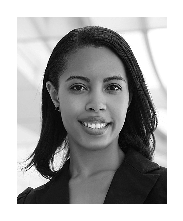
\includegraphics[width=1in,height=1.25in,clip,keepaspectratio]{a1.eps}}]{First A. Author} (M'76--SM'81--F'87) and all authors may include 
biographies. Biographies are often not included in conference-related
papers. This author became a Member (M) of IEEE in 1976, a Senior
Member (SM) in 1981, and a Fellow (F) in 1987. The first paragraph may
contain a place and/or date of birth (list place, then date). Next,
the author's educational background is listed. The degrees should be
listed with type of degree in what field, which institution, city,
state, and country, and year the degree was earned. The author's major
field of study should be lower-cased. 

The second paragraph uses the pronoun of the person (he or she) and not the 
author's last name. It lists military and work experience, including summer 
and fellowship jobs. Job titles are capitalized. The current job must have a 
location; previous positions may be listed 
without one. Information concerning previous publications may be included. 
Try not to list more than three books or published articles. The format for 
listing publishers of a book within the biography is: title of book 
(publisher name, year) similar to a reference. Current and previous research 
interests end the paragraph. The third paragraph begins with the author's 
title and last name (e.g., Dr.\ Smith, Prof.\ Jones, Mr.\ Kajor, Ms.\ Hunter). 
List any memberships in professional societies other than the IEEE. Finally, 
list any awards and work for IEEE committees and publications. If a 
photograph is provided, it should be of good quality, and 
professional-looking. Following are two examples of an author's biography.
\end{IEEEbiography}

\begin{IEEEbiography}[{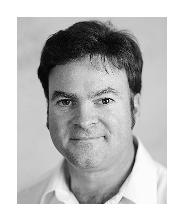
\includegraphics[width=1in,height=1.25in,clip,keepaspectratio]{a2.eps}}]{Second B. Author} was born in Greenwich Village, New York, NY, USA in 
1977. He received the B.S. and M.S. degrees in aerospace engineering from 
the University of Virginia, Charlottesville, in 2001.

Since 2009, he has been an Assistant Professor with the 
Mechanical Engineering Department, Texas A{\&}M University, College Station. 
He is the author of more than 150 articles. His research interests include high-pressure and high-density nonthermal plasma discharge processes and applications, plasma propulsion, and innovation plasma applications.

Dr. Author was a recipient of the International Association of Geomagnetism 
and Aeronomy Young Scientist Award for Excellence in 2008, and the IEEE 
Electromagnetic Compatibility Society Best Symposium Paper Award in 2011. 
\end{IEEEbiography}

\begin{IEEEbiography}[{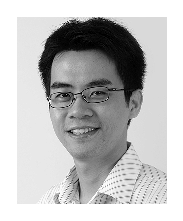
\includegraphics[width=1in,height=1.25in,clip,keepaspectratio]{a3.eps}}]{Third C. Author, Jr.} (M'87) received the B.S. degree in mechanical 
engineering from National Chung Cheng University, Chiayi, Taiwan, in 2004 
and the M.S. degree in mechanical engineering from National Tsing Hua 
University, Hsinchu, Taiwan, in 2006. He is currently pursuing the Ph.D. 
degree in mechanical engineering at Texas A{\&}M University, College 
Station, TX, USA.

From 2008 to 2009, he was a Research Assistant with the Institute of 
Physics, Academia Sinica, Tapei, Taiwan. His research interest includes the 
development of surface processing and biological/medical treatment 
techniques using nonthermal atmospheric pressure plasmas. 

Mr. Author's awards and honors include the Frew Fellowship (Australian 
Academy of Science), the I. I. Rabi Prize (APS), the European Frequency and 
Time Forum Award, the Carl Zeiss Research Award, the William F. Meggers 
Award and the Adolph Lomb Medal (OSA).
\end{IEEEbiography}

\EOD

\end{document}
